\section{Experimental Setup}

\subsection*{Circuit components}
    \begin{enumerate}
        \item Function Generator
        \item Oscilloscope
        \item Resistor (3.835 k$\Omega$)
        \item Capacitor (75 nF)
        \item Connecting wires
        \item Breadboard
    \end{enumerate}

    \subsection*{Circuit Diagram}

    \begin{figure}[H]
        \centering
        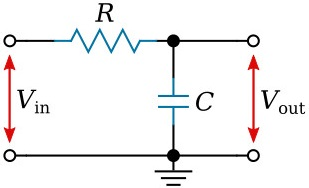
\includegraphics[width=0.8\columnwidth]{images/f2.jpg}
        \caption{Low-pass RC filter}
        \label{fig:5}
    \end{figure}

    \begin{figure}[H]
        \centering
        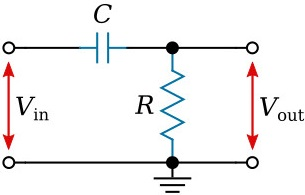
\includegraphics[width=0.8\columnwidth]{images/f1.jpg}
        \caption{High-pass RC filter}
        \label{fig:56}
    \end{figure}

\section{Data Analysis}

\subsection*{Low Pass Filter}
The following bode plots were obtained from the RC low pass filter circuit.

\begin{figure}[H]
        \centering
        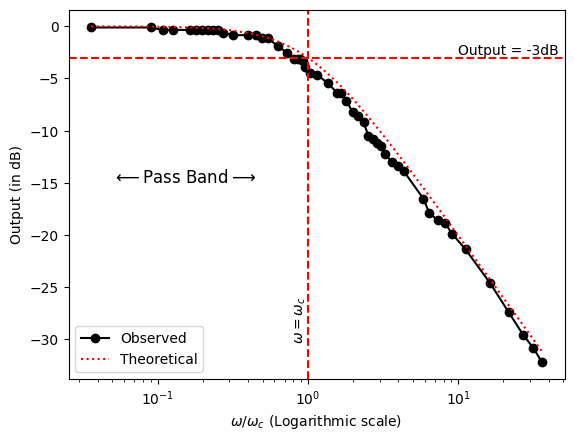
\includegraphics[width=0.9\columnwidth]{images/g1.png}
        \caption{Bode plot of $|H(j\omega)|_\text{dB}$ vs $\omega/\omega_c$ in a semi-log format for a low pass filter}
        \label{graph:1}
\end{figure}
    


As seen, the observed values of output gain closely matches the theoretical values. At $\omega = \omega_c$, the gain is $\approx -3$ dB as predicted. The gain is maximum ($\approx 1$) when $\omega << \omega_c$ which is effectively a low-pass filter. At higher frequencies, the output falls off with a roll-off of about -20 dB/decade.

\begin{figure}[H]
    \centering
    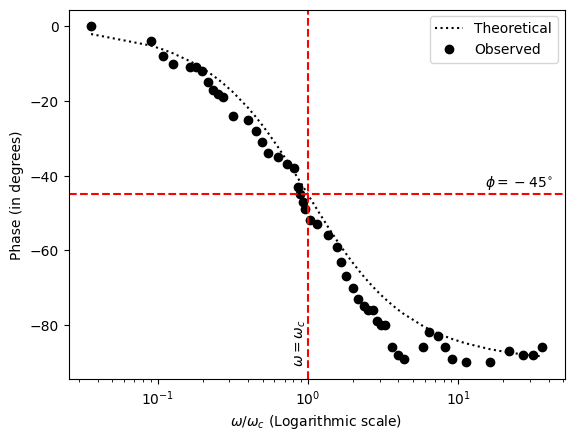
\includegraphics[width=0.9\columnwidth]{images/g2.png}
    \caption{Bode plot of $\phi$ vs $\omega/\omega_c$ in a semi-log format for a low pass filter}
    \label{graph:2}
\end{figure}


As predicted, At high frequencies, $\omega >> \omega_c$, $\phi \approx -90^{\circ}$ and at low frequencies, $\omega << \omega_c$, $\phi \approx 0^{\circ}$. And at cut-off frequency, $\phi \approx -45^{\circ}$. The heavy deviation observed at higher frequencies could be due to the high fluctuation observed in the oscilloscope. This can be due to fluctuations in the input signal or improper connections to the oscilloscope. 

\subsection*{High Pass Filter}
The following bode plots were obtained from the RC high pass filter circuit.

\begin{figure}[H]
    \centering
    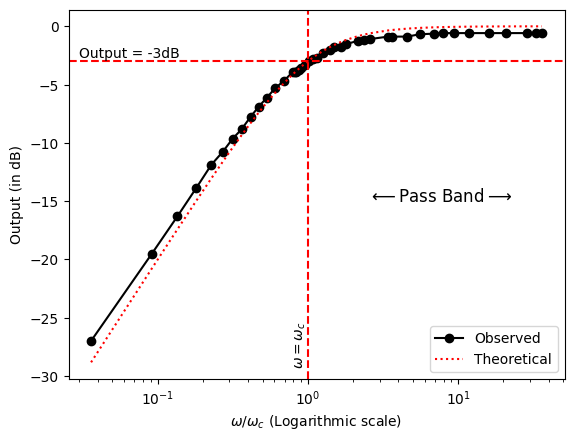
\includegraphics[width=0.9\columnwidth]{images/g3.png}
    \caption{Bode plot of $|H(j\omega)|_\text{dB}$ vs $\omega/\omega_c$ in a semi-log format for a high pass filter}
    \label{graph:3}
\end{figure}

As seen, the observed values of output gain closely matches the theoretical values. At $\omega = \omega_c$, the gain is $\approx -3$ dB as predicted. The gain is maximum ($\approx 1$) when $\omega >> \omega_c$ which is effectively a high-pass filter. At lower frequencies, the output falls off with a roll-off of about 20 dB/decade.

\begin{figure}[H]
    \centering
    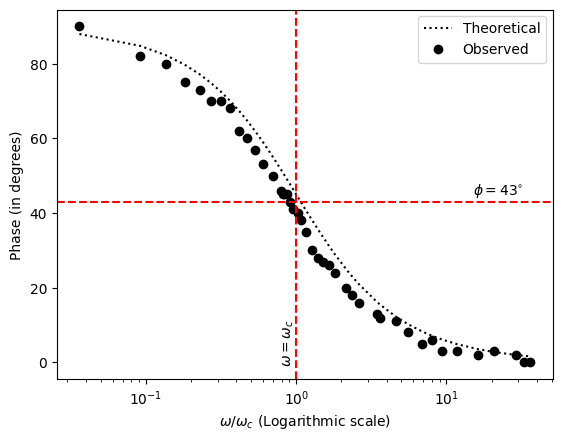
\includegraphics[width=0.9\columnwidth]{images/g4.png}
    \caption{Bode plot of $\phi$ vs $\omega/\omega_c$ in a semi-log format for a high pass filter}
    \label{graph:4}
\end{figure}

As predicted, At high frequencies, $\omega >> \omega_c$, $\phi \approx 0^{\circ}$ and at low frequencies, $\omega << \omega_c$, $\phi \approx 90^{\circ}$. And at cut-off frequency, $\phi \approx 45^{\circ}$